%%%%%%%%%%%%%%%%%%%%%%%%%%%%%%%%%%%%%%%%%
% Beamer Presentation
% LaTeX Template
% Version 1.0 (10/11/12)
%
% This template has been downloaded from:
% http://www.LaTeXTemplates.com
%
% License:
% CC BY-NC-SA 3.0 (http://creativecommons.org/licenses/by-nc-sa/3.0/)
%
%%%%%%%%%%%%%%%%%%%%%%%%%%%%%%%%%%%%%%%%%

%----------------------------------------------------------------------------------------
%	PACKAGES AND THEMES
%----------------------------------------------------------------------------------------

\documentclass{beamer}

\mode<presentation> {

% The Beamer class comes with a number of default slide themes
% which change the colors and layouts of slides. Below this is a list
% of all the themes, uncomment each in turn to see what they look like.

%\usetheme{default}
%\usetheme{AnnArbor}
%\usetheme{Antibes}
%\usetheme{Bergen}
%\usetheme{Berkeley}
%\usetheme{Berlin}
%\usetheme{Boadilla}
% \usetheme{CambridgeUS}
%\usetheme{Copenhagen}
%\usetheme{Darmstadt}
%\usetheme{Dresden}
%\usetheme{Frankfurt}
%\usetheme{Goettingen}
%\usetheme{Hannover}
%\usetheme{Ilmenau}
%\usetheme{JuanLesPins}
%\usetheme{Luebeck}
\usetheme{Madrid}
%\usetheme{Malmoe}
%\usetheme{Marburg}
%\usetheme{Montpellier}
% \usetheme{PaloAlto}
%\usetheme{Pittsburgh}
%\usetheme{Rochester}
%\usetheme{Singapore}
%\usetheme{Szeged}
%\usetheme{Warsaw}

% As well as themes, the Beamer class has a number of color themes
% for any slide theme. Uncomment each of these in turn to see how it
% changes the colors of your current slide theme.

%\usecolortheme{albatross}
%\usecolortheme{beaver}
%\usecolortheme{beetle}
%\usecolortheme{crane}
%\usecolortheme{dolphin}
%\usecolortheme{dove}
%\usecolortheme{fly}
%\usecolortheme{lily}
%\usecolortheme{orchid}
\usecolortheme{rose}
%\usecolortheme{seagull}
%\usecolortheme{seahorse}
%\usecolortheme{whale}
%\usecolortheme{wolverine}

%\setbeamertemplate{footline} % To remove the footer line in all slides uncomment this line
%\setbeamertemplate{footline}[page number] % To replace the footer line in all slides with a simple slide count uncomment this line

%\setbeamertemplate{navigation symbols}{} % To remove the navigation symbols from the bottom of all slides uncomment this line
}

\usepackage{graphicx} % Allows including images
\graphicspath{{./fig/}}
\DeclareGraphicsExtensions{.pdf,.jpeg,.png}
\usepackage{booktabs} % Allows the use of \toprule, \midrule and \bottomrule in tables
\usepackage[numberedbib]{apacite}
\usepackage{ amssymb }

%----------------------------------------------------------------------------------------
%	TITLE PAGE
%----------------------------------------------------------------------------------------

\title[cvx + sgd] {
    Convex Learning Problems and Stochastic Gradient Descent
    \vspace{5mm}
    (ML Reading, UQ)
}

\author{Vektor Dewanto} % Your name
\institute[RDL, UQ] % Your institution as it will appear on the bottom of every slide, may be shorthand to save space
{
% Affiliation: RDL, UQ\\ % Your institution for the title page
\medskip
\textit{vektor.dewanto@gmail.com } % Your email address
}
\date{\today} % Date, can be changed to a custom date

\begin{document}

\begin{frame}
\titlepage % Print the title page as the first slide
\end{frame}

\begin{frame}
\frametitle{Outline} % Table of contents slide, comment this block out to remove it
\tableofcontents % Throughout your presentation, if you choose to use \section{} and \subsection{} commands, these will automatically be printed on this slide as an overview of your presentation
\end{frame}

%----------------------------------------------------------------------------------------
%	PRESENTATION SLIDES
%----------------------------------------------------------------------------------------
%%%%%%%%%%%%%%%%%%%%%%%%%%%%%%%%%%%%%%%%%%%%%%%%%%%%%%%%%%%%%%%%%%%%%%%%%%%%%%%
\section{Convexity, Lipschitzness, and Smoothness}
\frame{\tableofcontents[currentsection, hideothersubsections]}


\begin{frame}
\frametitle{Convexity: Convex sets}

\begin{figure}
    \centering
    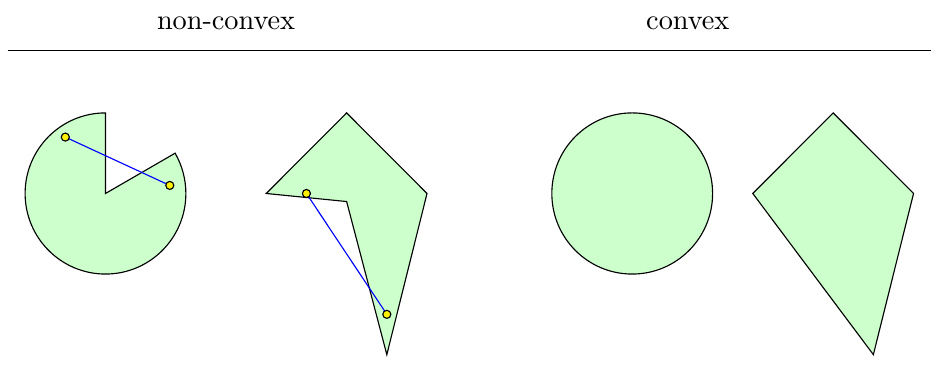
\includegraphics[scale=0.35]{cvx_noncvx}
\end{figure}

\begin{figure}
    \centering
    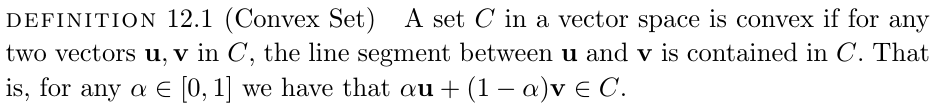
\includegraphics[scale=0.4]{cvx_set}
\end{figure}

\end{frame}

\begin{frame}
\frametitle{Convexity: Convex functions}

\begin{figure}
    \centering
    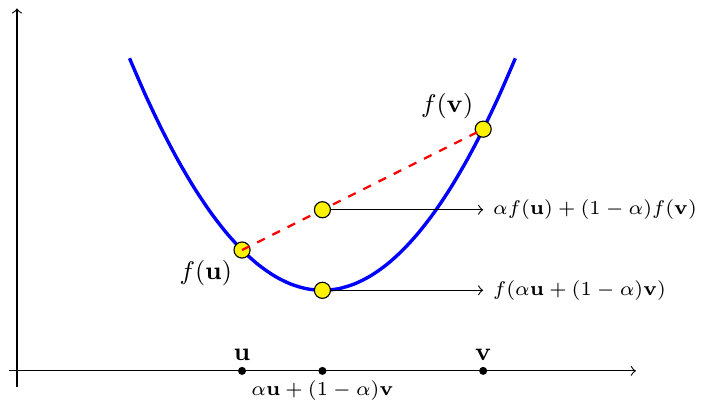
\includegraphics[scale=0.35]{cvx_fn}
\end{figure}

\begin{figure}
    \centering
    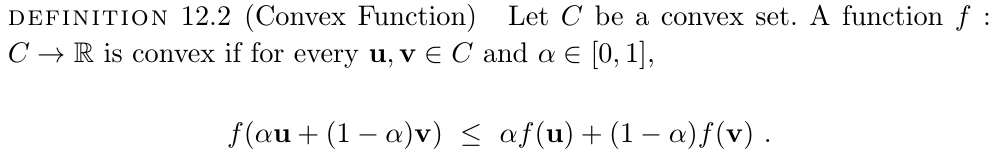
\includegraphics[scale=0.4]{cvx_fn_def}
\end{figure}

\end{frame}

\begin{frame}
\frametitle{Convexity: Convex functions}

Properties:
\begin{itemize}
    \item  every local minimum is also a global minimum
    \item  for every $\mathbf{w}$ we can construct a tangent to $f$
    at $\mathbf{w}$ that lies below $f$ everywhere.
    If f is differentiable, this tangent is the linear function
    % $l(u) = f(w) + h∇f (w), u − wi$
\end{itemize}

\begin{figure}
    \centering
    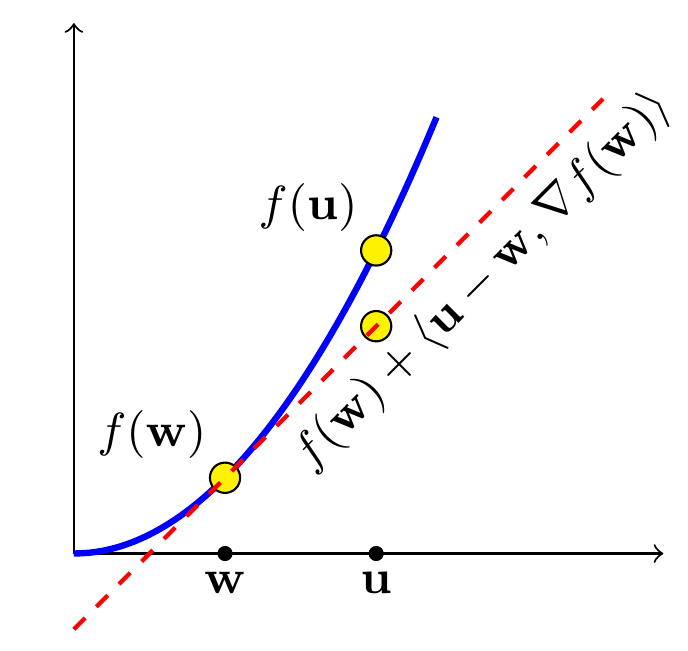
\includegraphics[scale=0.25]{cvx_fn_tangent}
\end{figure}

\end{frame}

\begin{frame}
\frametitle{Convexity: Convex functions}

\begin{figure}
    \centering
    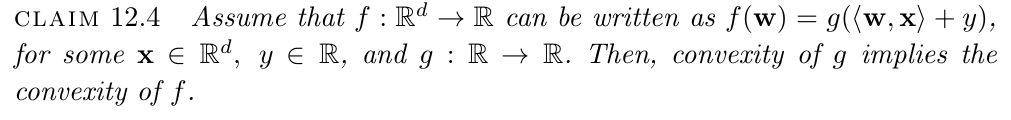
\includegraphics[scale=0.4]{claim_12_4}
\end{figure}

\begin{figure}
    \centering
    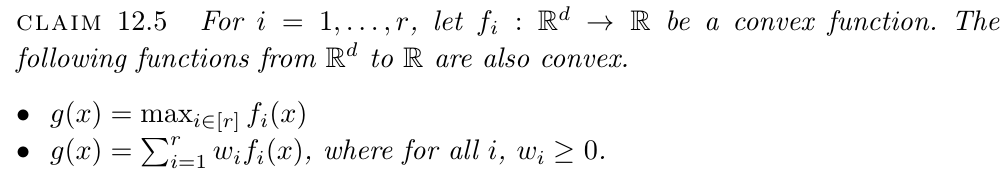
\includegraphics[scale=0.4]{claim_12_5}
\end{figure}

\end{frame}


\begin{frame}
\frametitle{Lipschitzness}
\begin{figure}
    \centering
    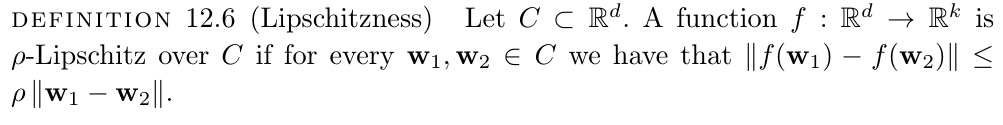
\includegraphics[scale=0.4]{def_12_6}
\end{figure}

\begin{itemize}
    \item a Lipschitz function cannot change too fast
    \item if the derivative of $f$ is everywhere bounded (in absolute value) by $\rho$,
        then the function is $\rho$-Lipschitz.
    \item composition of Lipschitz functions preserves Lipschitzness.
\end{itemize}

\end{frame}


\begin{frame}
\frametitle{Smoothness}
\begin{figure}
    \centering
    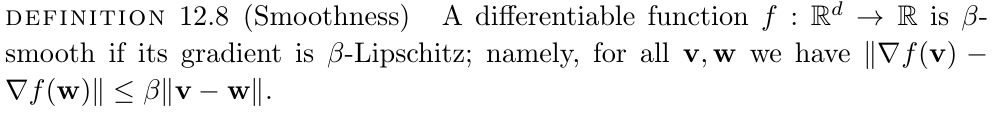
\includegraphics[scale=0.4]{def_12_8}
\end{figure}

\begin{itemize}
    \item when a function is both convex and smooth,\\
        we have both upper and lower bounds on the difference between
        the function and its first order approximation.
    \item a composition of a smooth scalar function over a linear function preserves smoothness.
\end{itemize}

\end{frame}

\section{Convex Learning Problems}
\frame{\tableofcontents[currentsection, hideothersubsections]}

In general, a convex learning problem is a problem whose hypothesis class is a
convex set, and whose loss function is a convex function for each example.

Convex-Smooth/Lipschitz-Bounded
problems are learnable.

\section{Surrogate Loss Function}
\frame{\tableofcontents[currentsection, hideothersubsections]}

\begin{frame}
\frametitle{Surrogate Loss Fn: Intro}

WHAT:\\
handle some nonconvex problems
by minimizing “surrogate” loss functions that are convex
\vspace{2mm}

WHY:\\
the natural loss function is not convex
\vspace{2mm}

HOW:\\
to upper bound the nonconvex loss function by a convex surrogate loss function.
the requirements from a convex surrogate loss are as follows:
\begin{itemize}
    \item It should be convex.
    \item It should upper bound the original loss.
\end{itemize}
\end{frame}

\begin{frame}
\frametitle{Surrogate Loss Fn: Example}
example:
learning the hypothesis class of half-
spaces with respect to the 0 − 1 loss.

For example, in the context of learning halfspaces, we can define the so-called
hinge loss as a convex surrogate for the 0 − 1 loss, as follows:

\end{frame}




% \begin{frame} [allowframebreaks]
\frametitle{References}
{\tiny
\bibliographystyle{apacite}
\bibliography{ref}
}
\end{frame}

\begin{frame}
\Huge{\centerline{Discussion time and thank you.}}
\end{frame}

%%%%%%%%%%%%%%%%%%%%%%%%%%%%%%%%%%%%%%%%%%%%%%%%%%%%%%%%%%%%%%%%%%%%%%%%%%%%%%%

\end{document}
